\chapter{State Estimation}
\label{ch:st_est}
State estimation is the principle of estimating the internal state of the system from the measurement of inputs and outputs of the system. In general knowledge of the internal state of the system will make the system easy to control. Figure \ref{fig:observer} shows the usage of state estimator in state feedback control loop.
\begin{figure}[h]
  \centering
  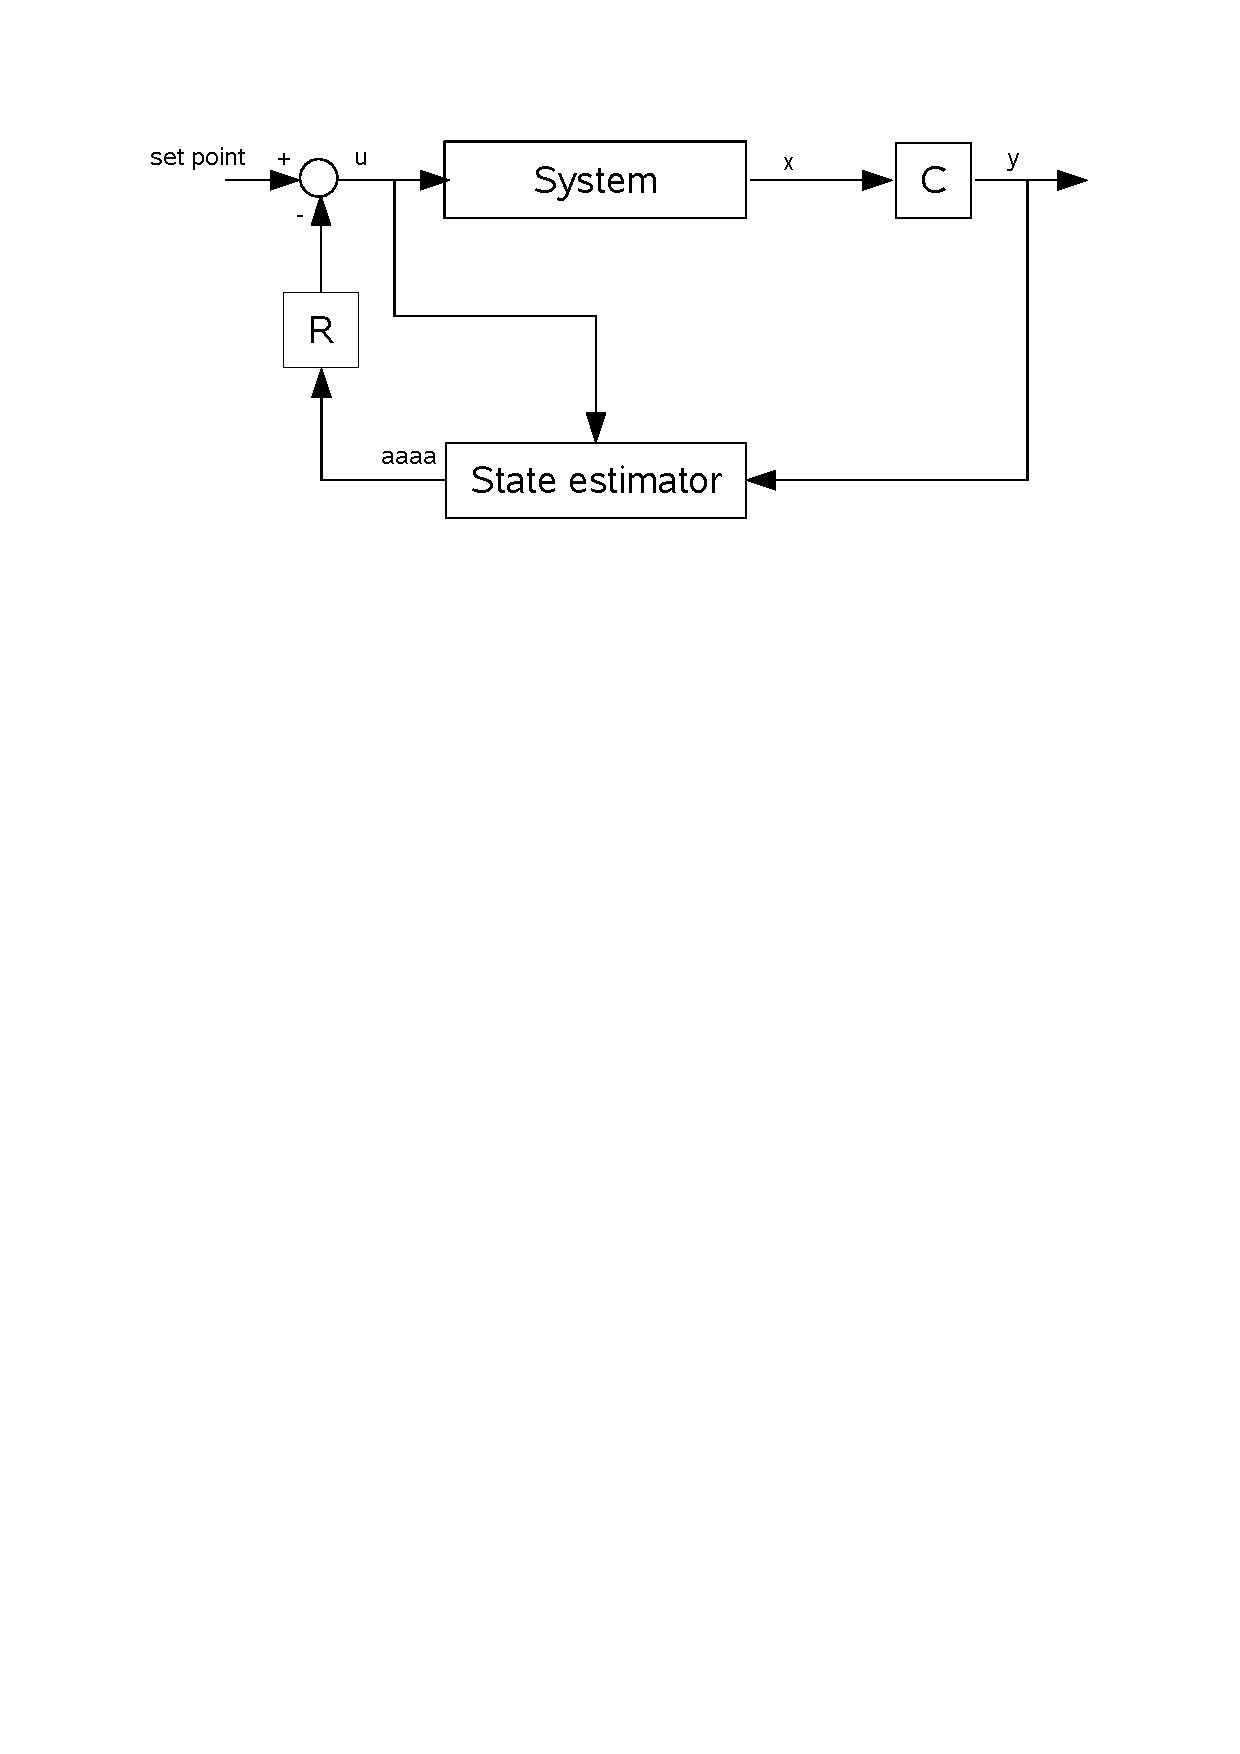
\includegraphics[trim = 10mm 200mm 20mm 20mm, clip,scale=0.80]{Bilder/system_observer.pdf}
  \caption{Structure of state feedback controller with state estimator}
  \label{fig:observer}
\end{figure}

A general nonlinear system in state space form,
\begin{equation}
\begin{split}
\label{eqn:nl_sys}
\dot{x}(t) &= f(x(t),u(t)) , x(t=0) = x_0 \\
y(t) &= g(x(t),u(t))
\end{split}
\end{equation}

In Equation \ref{eqn:nl_sys}, \emph{x(t)} represents the vector of internal states, \emph{u(t)} represents the vector of inputs and \emph{y(t)} represents the vector of outputs of the system. $x_0$ is the initial state of the system which is usually unknown. 
The state estimator is described by the system equation with additional correction term
\begin{equation}
\begin{split}
\label{eqn:est_sys}
\dot{\hat{x}}(t) &= f(\hat{x}(t),u(t)) + K(y(t)-\hat{y}(t)) , \hat{x}(t=0) = \hat{x}_0\\
\hat{y}(t) &= g(\hat{x}(t),u(t))
\end{split}
\end{equation}
$\hat{x}(t)$ is the state vector of estimator and \emph{K} is the gain matrix.  A state estimator should satisfy the following properties
\begin{itemize}
\item \textbf{Simulation property:} For the same initial condition $x(t_0) = \hat{x}_0$ of the estimator and the system to be observed, then it holds that $x(t) = \hat{x}(t) \forall t > 0 $.
\item \textbf{Convergence property:} If $x(t_0) \neq \hat{x}_0$, then $x(t) - \hat{x}(t)$ tends to zero as $ t \rightarrow \infty $
\end{itemize}

The different approaches for state estimator design differs in the calculation of gain matrix \emph{K} in Equation \ref{eqn:est_sys}.
